% !TeX spellcheck = fr_FR

% TODO: Replace scan images with clean text where possible

\documentclass[a4paper, 10pt]{report}

\usepackage[french]{babel}
\usepackage[T1]{fontenc}

\usepackage{amsmath, amssymb, amsfonts}

\usepackage{hyperref}
\usepackage{geometry}

\usepackage{xcolor}
\usepackage{graphicx}

\usepackage{fancyhdr}
\usepackage{lastpage}

\usepackage{enumitem}

\geometry{
	a4paper,
	left=25mm,
	right=25mm,
	top=35mm,
	bottom=25mm,
	headsep=5mm,
	headheight=20mm,
}

\definecolor{solution}{HTML}{E5E4E2}
\providecommand{\abs}[1]{\lvert#1\rvert}
\providecommand{\norm}[1]{\lVert#1\rVert}
\DeclareMathOperator{\card}{card}

\begin{document}
	
	\renewcommand{\headrule}{%
		\vspace{-4pt}\hrulefill
		\raisebox{-6.8pt}{\ 
\includegraphics[height=5mm]{../../icon.png}}
		\hrulefill
	}	
	\pagestyle{fancy}
	\fancyhf{}
	
	\fancyhead[L]{\small \slshape Automne 2024}
	\fancyhead[C]{\Large \bfseries Analyse I - Série 05}
	\fancyhead[R]{\small Buff Mathias}
	\fancyfoot[L]{
		\small Source files available at:
		\href{https://github.com/MathiasBuff/bsc-math}
		{github.com/MathiasBuff/bsc-math}
	}
	\fancyfoot[R]{
		\small Page \thepage
		\hspace{1pt} /
		\pageref*{LastPage}
	}
	

	\noindent
	\textbf{Exercice 1.} Soient $a < b$ deux réels positifs.
	Définissons les deux suites $(x_n)$ et $(y_n)$ par récurrence
	par $x_0 = a, y_0 = b$ et pour tout $n \in \mathbb{N},
		x_{n+1} = \sqrt{x_ny_n}$ et $y_{n+1} = \frac{x_n + y_n}{2}$.
	\begin{enumerate}[label=(\roman*)]
		\item Montrer que pour tout $x, y \in \mathbb{R}, x^2 + y^2
			\geq 2xy$. En déduire que $x_n \leq y_n$ pour tout
		$n \in \mathbb{N}$.
		%
		\item Montrer que $(x_n)$ croît et que $(y_n)$ décroît.
		%
		\item Montrer que $(x_n)$ et $(y_n)$ convergent (on notera
		leurs limites $\ell$ et $\ell'$). Utiliser le fait que
		$y_{n+1} = \frac{x_n + y_n}{2}$ afin de montrer que
		$\ell' = \frac{\ell + \ell'}{2}$. En déduire que $\ell = \ell'$.
	\end{enumerate}
	\textit{La limite commune est appelée moyenne arithmético-géométrique
		de $a$ et $b$.}.\\
	
	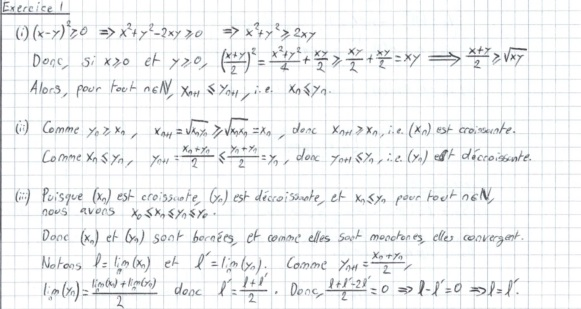
\includegraphics{ex01.jpg}
	
	\vspace{5mm}
	\noindent
	\textbf{Exercice 2.} Soit $\Phi: \mathbb{N} \to \mathbb{N}$ une
	fonction strictement croissante. Montrer que $\Phi(n) \geq n$
	pour tout $n \in \mathbb{N}$.\\
	
	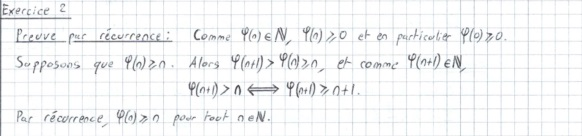
\includegraphics{ex02.jpg}	
	
	\vspace{5mm}
	\noindent
	\textbf{Exercice 3.} Montrer que toute sous-suite extraite d'une
	suite convergente a la même limite.\\
	
	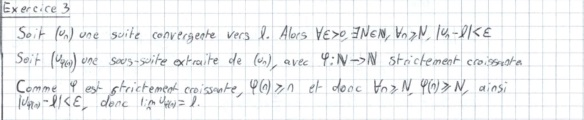
\includegraphics{ex03.jpg}
	
	\newpage
	
	\fancyhf{}
	\renewcommand{\headrule}
	{\rule{\textwidth}{0pt}}
	\fancyfoot[R]{
		\small Page \thepage
		\hspace{1pt} /
		\pageref*{LastPage}
	}
	
	\noindent
	\textbf{Exercice 4.} Soit $(u_n)$ une suite et définissons
	$v_n := \sup_{k \geq n}u_k$. Montrer que la suite $(v_n)$ est
	décroissante.\\
	
	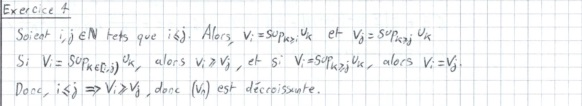
\includegraphics{ex04.jpg}
	
	\vspace{5mm}
	\noindent
	\textbf{Exercice 5.} Soit $(u_n)$ une suite bornée. Montrer que
	$(u_n)$ converge si et seulement si \[\limsup_n{u_n} = \liminf_n{u_n}\]
	et que dans ce cas ce nombre est égal à $\lim_n{u_n}$.\\
	
	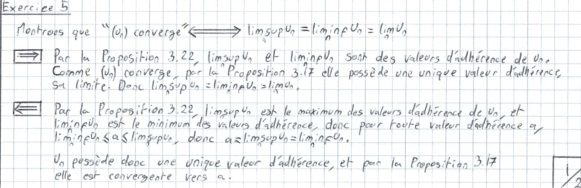
\includegraphics{ex05.jpg}
	
	\vspace{5mm}
	\noindent
	\textbf{Exercice 6.} 
	\begin{enumerate}[label=(\roman*)]
		\item Donner un exemple de suites possédant respectivement
		une, deux, et trois valeurs d'adhérence.
		\item Même question avec $m$ valeurs d'adhérence.
		\item Même question avec $\mathbb{N}$ comme ensemble des
		valeurs d'adhérence.
	\end{enumerate}
	Déterminer, lorsqu'elles existent, les $\liminf$ et $\limsup$
	de ces suites.\\
	
	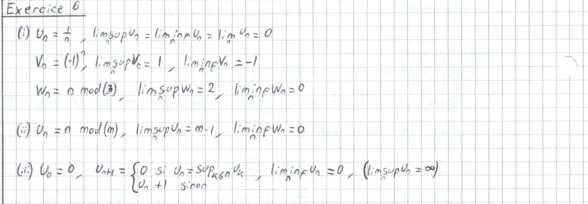
\includegraphics{ex06.jpg}
	\colorbox{solution}
	{\begin{minipage}{0.9\textwidth}
		\textit{\color{blue} Est-ce qu'il serait plus correct de
			dire que $\limsup$ n'existe pas pour la suite du point
			(iii) ?}\\
	\end{minipage}}
	
	\newpage
	
	\noindent
	\textbf{Exercice 7.} Soient $(u_n)$ et $(v_n)$ deux suites telles
	que $\exists K \in \mathbb{N}, \forall n \geq K, u_n = v_n$.
	\begin{enumerate}[label=(\roman*)]
		\item Soit $(u_n)$ convergente. Montrer que
		$\lim_n{u_n} = \lim_n{v_n}$.
		\item Soit $(u_n)$ bornée. Montrer que\\[-1em]
		\[
			\limsup_n{u_n} = \limsup_n{v_n}, \qquad
			\liminf_n{u_n} = \liminf_n{v_n}.
		\]\\[-3em]
	\end{enumerate}
	Cet exercice montre que les notions de $\lim, \limsup$ et $\liminf$
	ne dépendent que du comportement asymptotique de la suite.\\
	
	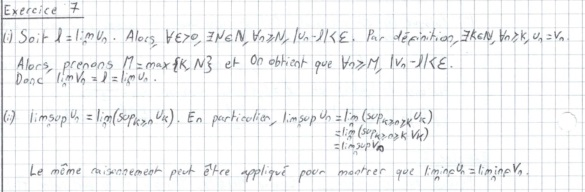
\includegraphics{ex07.jpg}
	
	\vspace{5mm}
	\noindent
	\textbf{Exercice 8.} (Théorème de Cesàro)
	Soit $(u_n)_{n \in \mathbb{N}*}$ une suite convergeant vers $\ell$.
	Posons $S_n = u_1 + \dotso + u_n$. Nous désirons montrer le théorème
	de Cesàro, c'est-à-dire que $\frac{1}{n}S_n$ converge vers $\ell$. 
	\begin{enumerate}[label=(\roman*)]
		\item Montrer que pour tout $\varepsilon > 0$, il existe
		$N \in \mathbb{N}$ tel que pour tout $n \geq N$,
		\[\left|\sum_{k=N}^{n}u_k - (n - N + 1)\ell\right| < (n - N + 1)\varepsilon\]
		%
		\item Montrer que pour tout $\varepsilon > 0$ et $N \in \mathbb{N}$,
		il existe $N' \geq N$ tel que pour tout $n \geq N'$,
		\[\frac{1}{n}\left|\sum_{k=1}^{N-1}u_k\right| < \varepsilon\]
		%
		\item Montrer, en découpant la somme $S_n$ astucieusement, que
		$\frac{1}{n}S_n$ converge vers $\ell$.\\
	\end{enumerate}
	
	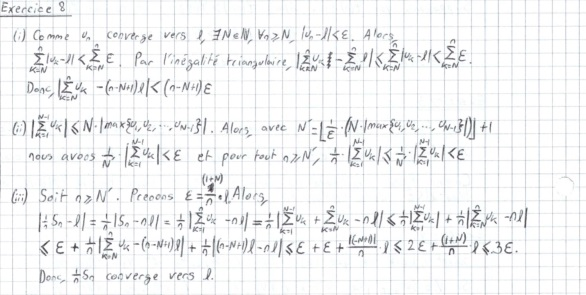
\includegraphics{ex08.jpg}
	
	
%	
%	
%	\colorbox{solution}
%	{
%		\begin{minipage}{0.9\textwidth}
%			s
%		\end{minipage}
%	}
%	
%	\colorbox{solution}
%	{
%		\begin{minipage}{0.9\textwidth}
%			\begin{enumerate}[label=(\alph*)]
%				\item a
%			\end{enumerate}
%		\end{minipage}
%	}
	
\end{document}
